\documentclass{beamer}

\usepackage{graphics}
\usepackage{graphicx}
\usepackage{amsmath,amssymb,amsthm}
%\usepackage{subeqnarray}
%\usepackage{easybmat}
%\usepackage{subfigure}



%\usepackage{HA-prosper}
%\usepackage[dvips,letterpaper]{geometry}

\def\Proba#1{\mathcal{P}\left(#1\right)}
\def\Surv{\mathcal{S}}
\def\R{\mathcal{R}}
\def\D{\mathcal{D}}
\def\C{\mathcal{C}}
\def\M{\mathcal{M}}
\def\L{\mathcal{L}}
\def\IC{\mathbb{C}}
\def\IN{\mathbb{N}}
\def\IR{\mathbb{R}}
\def\IZ{\mathbb{Z}}
\def\IK{\mathbb{K}}
\def\II{\mathbb{I}}
\def\Rzero{\mathcal{R}_0}
\newcommand{\diag}{\operatorname{diag}}
\def\tr{\textrm{tr}}
\def\det{\textrm{det}}
\def\sgn{\textrm{sgn}}
\def\imply{$\Rightarrow$}
\def\dbint{\int\!\!\!\int}
\def\dbintb{\mathop{\int\!\!\!\!\int}}
\def\tpint{\int\!\!\!\int\!\!\!\int}

\def\red{\color[rgb]{1,0,0}}

\newtheorem{proposition}{Proposition}

\setbeamertemplate{navigation symbols}{}
\setbeamertemplate{footline}
{%
\quad\insertsection\hfill p. \insertpagenumber\quad\mbox{}\vskip2pt
}

\title[Midterm]{Midterm}
\date{}

\begin{document}
%%%%%%%%%%%%%%
%%%%%%%%%%%%%%


\section{Exercise 1}

\frame{\frametitle{Exercise 1}
We have the following setup:
a tank contains initially, at time $t=0$, 500 litres of water. There is an inflow, at the rate of $r_{in}$ litres per minute, and an outflow at the rate of $r_{out}$ litres per minute. Before the experiment starts, the tank contains a concentration of salt of $C_0$. At the start of the experiment, liquid starts flowing into the tank, and the contents of the tank start flowing out.
\begin{center}
\includegraphics[width=0.45\textwidth]{fig1_midterm2007}
\end{center}
}

\frame{\frametitle{Exercise 1 (cont.)}
{\bf 1.a.}
Write a differential equation for the variation of the volume $V(t)$ of liquid in the tank at time $t$.

\noindent
{\bf 1.b.} 
Find the expression of $V(t)$, the volume of liquid in the tank at time $t$.

\noindent
{\bf 1.c.} Assume that $r_{in}=10$ litres per minute. What is the value of $r_{out}$, if after 1 hour, there remains exactly 100 litres of liquid in the tank.
}

\frame{\frametitle{Exercise 1 (cont.)}
\noindent
{\bf 1.d.} Assume now that $r_{in}=r_{out}$, so that the amount of liquid remains constant in the tank. Denote $r(t)$ this rate of in/out-flow, which we assume can vary with time. The inflow contains a concentration $S_0$ of salt. Assuming that the tank is well stirred, so that the concentration of salt is uniform in the tank, write a differential equation for the concentration $C(t)$ of salt in the tank at time $t$.

\noindent
{\bf 1.e.}
The general solution to the linear equation $x'+p(t)x=q(t)$ is given by 
\[
x(t)=e^{-\int p(t)dt}\left(\int e^{\int p(t)dt}q(s)ds+K\right),\quad K\in\mathbb{R}.
\]
Using this, solve the differential equation you found in {\bf 1.d}, with the initial condition $C(0)=C_0$.
}

\section{Exercise 2}

\frame{\frametitle{Exercise 2}
\noindent
{\bf 2.} Consider the difference equation
\begin{equation}\label{eq:1}
x_{t+1}=\frac{ax_t}{b+x_t},
\end{equation}
with $a,b>0$ and $x_0\geq 0$.

\noindent{\bf 2.a.} Show that for $x_0\geq 0$, $x_t\geq 0$ for all $t$.

\noindent{\bf 2.b.} Find the fixed points of \eqref{eq:1}. 

\noindent{\bf 2.c.} Study the relevance (nonnegativity) and stability of these fixed points, as a function of the (relative) values of $a$ and $b$.
}

\frame{
\noindent{\bf 2.d.} Summarize your findings of {\bf 2.c} in a diagram having $a$ on the $x$-axis (assuming a fixed value of $b$), and the value of the fixed points on the $y$-axis, as shown in Figure~\ref{fig:2}. Indicate an attracting equilibrium by a thick line, a repelling one by a dashed line.
\begin{figure}[htbp]
\begin{center}
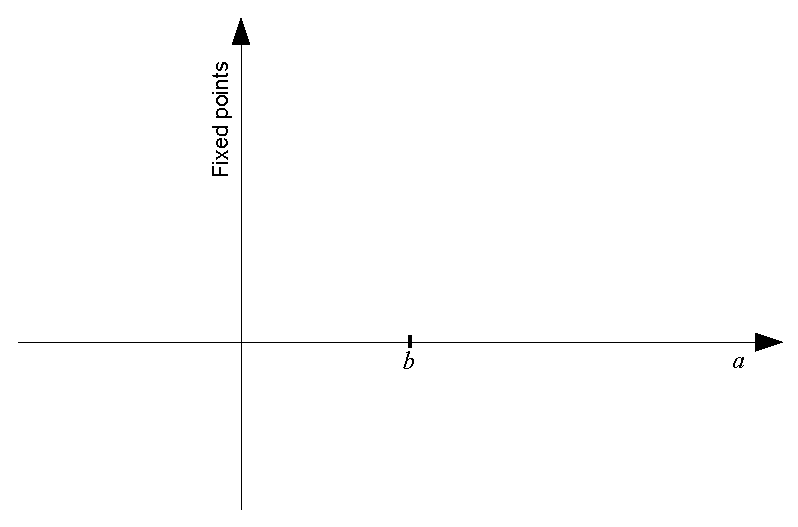
\includegraphics[width=0.45\textwidth]{fig2_midterm2007}
\caption{Setup of the bifurcation diagram for exercise {\bf 2.d}.}
\label{fig:2}
\end{center}
\end{figure}


\noindent{\bf 2.e.} Can \eqref{eq:1} have period 2 points other than its fixed points?
}

\section{Exercise 3}
\frame{\frametitle{Exercise 3}
Consider the following model for hares and fox, where $H(t)$ and $F(t)$ are the numbers of hares and fox at time $t$, respectively.
\begin{equation}\label{eq:2}
\begin{aligned}
H' &= (b_H-d_H)H - \pi HF \\
F' &= \sigma\pi HF -d_FF.
\end{aligned}
\end{equation}
The parameters are $b_H$, birth rate of hares, $d_H$, death rate of hares, $d_F$, death rate of fox, $\pi$, the predation rate, and $\sigma$, the conversion coefficient. We assume that $b_H,d_H,d_F>0$, while $\pi\geq 0$ and 
$0\leq\sigma\leq 1$. System \eqref{eq:2} is considered together with initial conditions $(H(0),F(0))=(H_0,F_0)$, with $H_0,F_0>0$.

\noindent{\bf 3.a.}
Suppose that there is no predation, i.e., $\pi=0$. Solve system \eqref{eq:2}, and discuss the behavior of its solutions as a function of the relative values of $b_H$ and $d_H$.

\noindent{\bf 3.b.}
Suppose now that $\pi>0$ and $\sigma>0$. Draw the nullclines of \eqref{eq:2}; show the direction field in each region of $\mathbb{R}_+^2$ hence delimited; identify the equilibria.
}

\frame{
\noindent{\bf 3.c.}
Discuss the relevance (nonnegativity) and local stability of the equilibria, as a function of the relative values of $b_H$, $d_H$ and $d_F$, in the $\pi,\sigma>0$ case.
}

\end{document}